\begin{example}[Geodésicas en $\mathbb{H}^{2}$]
	Consideremos al subconjunto de $\mathbb{R}^2$:
	\[
		\mathbb{H}^{2} = \{(x,y): x \in \mathbb{R}, y > 0\}
	\]
	es evidente que este subconjunto es abierto, y, con la topología heredada de $\mathbb{R}^{2}$ será una variedad suave. Dotaremos a $\mathbb{H}^{2}$ con la métrica cuyos coeficientes son:
	\[
		g_{ij} = \frac{R\delta_{ij}}{y^{2}},
	\]
	donde $R$ es una constante real positiva. Para calcular las geodésicas comenzaremos encontrando la inversa de la matriz asociada a esta métrica, esto es sencillo dado que tenemos una matriz diagonal de $2 \times 2$,
	\[
		G = \begin{bmatrix}
			\frac{R}{y^2} & 0             \\[12pt]
			0             & \frac{R}{y^2}
		\end{bmatrix},
		\qquad
		G^{-1} = \begin{bmatrix}
			\frac{y^2}{R} & 0               \\[12pt]
			0             & \frac{y^{2}}{R}
		\end{bmatrix}
	\]
	Ahora, utilizando la fórmula que hemos encontrado para calcular los símbolos de Christoffel tendremos:
	\begin{align*}
		\Gamma_{ij}^{m} & = \frac{1}{2} \sum_{k=1}^{2}
		(\partial_{i}g_{jk} + \partial_{j}g_{ki} - \partial{k}g_{ij}) g^{km} \\
		                & = \frac{1}{2} \left[
		(\partial_{i}g_{j1} + \partial_{j}g_{1i} - \partial_{1}g_{ij})g^{1m} + (\partial_{i}g_{j2} + \partial_{j}g_{2i} - \partial_{2}g_{ij})g^{2m}
		\right]
	\end{align*}
	Notemos que muchos de los términos en esta expresión son nulos, dado que las matrices son diagonales, se tendrá que $g_{12} = g_{21} = g^{12} = g^{21} = 0$. Además, como $\partial_{1} = \frac{\partial}{\partial x}$, se tendrá que $\partial_{1} g_{ij} = 0$. Por lo tanto, tendremos que los símbolos de Christoffel son:
	\begin{align*}
		\Gamma_{11}^{1} & = \frac{1}{2}\left[
		(\partial_{1}g_{11} + \partial_{1}g_{11} - \partial_{1}g_{11})g^{11}
		+ (\partial_{1}g_{12} + \partial_{1}g_{21} - \partial_{2}g_{11})g^{21}
		\right] = 0                                                                     \\
		\Gamma_{11}^{2} & = \frac{1}{2}\left[
		(\partial_{1}g_{11} + \partial_{1}g_{11} - \partial_{1}g_{11})g^{12}
		+ (\partial_{2}g_{12} + \partial_{2}g_{21} - \partial_{2}g_{11})g^{22}
		\right]                                                                         \\
		                & = \frac{1}{2}(-\partial_{2}g_{11})g^{22} = \frac{1}{2}\left(
		-\frac{\partial}{\partial y} \frac{R}{y^{2}}
		\right) \frac{y^2}{R} = \frac{1}{y}                                             \\
		\Gamma_{12}^{1} & = \frac{1}{2} \left[
		(\partial_{1}g_{21} + \partial_{2}g_{11} - \partial_{1}g_{12})g^{11}
		+ (\partial_{1}g_{22} + \partial_{2}g_{21} - \partial_{2}g_{12})g^{21}
		\right]                                                                         \\
		                & = \frac{1}{2} (\partial_{2}g_{11})g^{11} = \frac{1}{2} \left(
		\frac{\partial}{\partial y} \frac{R}{y^2} \right) \frac{y^2}{R}
		= - \frac{1}{y} =\Gamma_{21}^{1}                                                \\
		\Gamma_{12}^{2} & = \frac{1}{2} \left[
		(\partial_{1}g_{21} + \partial_{2}g_{11} - \partial_{1}g_{12})g^{12}
		+ (\partial_{1}g_{22} + \partial_{2}g_{21} - \partial_{2}g_{12})g^{22}
		\right] = 0 = \Gamma_{21}^{2}                                                   \\
		\Gamma_{22}^{1} & = \frac{1}{2} \left[
		(\partial_{2}g_{21} + \partial_{2}g_{12} - \partial_{1}g_{22})g^{11}
		+ (\partial_{2}g_{22} + \partial_{2}g_{22} - \partial_{2}g_{22})g^{21}
		\right] = 0                                                                     \\
		\Gamma_{22}^{2} & = \frac{1}{2} \left[
		(\partial_{2}g_{21} + \partial_{2}g_{12} - \partial_{1}g_{22})g^{12}
		+ (\partial_{2}g_{22} + \partial_{2}g_{22} - \partial_{2}g_{22})g^{22}
		\right]                                                                         \\
		                & = \frac{1}{2} (\partial_{2}g_{22})g^{22} = \frac{1}{2} \left(
		\frac{\partial}{\partial y} \frac{R}{y^2} \right) \frac{y^2}{R}
		= - \frac{1}{y}
	\end{align*}
	Si $\gamma$ es una geodésica podemos suponer que está parametrizada como $\gamma(t) = (x(t),y(t))$, por cuestiones de notación omitiremos el parámetro $t$ y escribiremos simplemente $\gamma = (x,y)$; el sistema de ecuaciones geodésicas quedará de la siguiente forma:
	\begin{align*}
		x'' + \Gamma_{11}^{1} (x')^2 + \Gamma_{12}^{1} x'y' + \Gamma_{21}^{1}x'y' + \Gamma_{22}^{1}(y')^{2} & = 0 \\
		y'' + \Gamma_{11}^{2} (x')^2 + \Gamma_{12}^{2} x'y' + \Gamma_{21}^{2}x'y' + \Gamma_{22}^{2}(y')^{2} & = 0
	\end{align*}
	este sistema se reduce a:
	\[
		\begin{cases}
			x'' - \frac{2}{y} x'y'                         & = 0 \\[12pt]
			y'' + \frac{1}{y} (x')^2 - \frac{1}{y}(y')^{2} & = 0
		\end{cases}
	\]
	Resolveremos este sistema de ecuaciones diferenciales por casos. Primero supongamos que $x' \neq 0$, esto implica que $x = x_{0}$, donde $x_0$ es una constante. Esto reducirá el sistema de ecuaciones de tal modo que simplemente se deberá encontrar la solución a la ecuación diferencial no lineal de segundo orden:
	\[
		y'' - \frac{1}{y}(y')^{2} = 0
	\]
	esta ecuación diferencial tiene por solución $y = y_0 e^{kt}$, donde $y_0$ y $k$ son constantes. Esto quiere decir que cuando $x = x_0$ sea una constante las geodésicas será una curva de la forma $\gamma(t) = (x_0, y_0 e^{kt})$.

	Por otro lado, supongamos que $x'(t) \neq 0$. Notemos que si $\gamma$ es una geodésica, entonces $\|\gamma'(t)\|$ es una constante, esto es una sencilla consecuencia, por la compatibilidad de la métrica con la conexión:
	\begin{align*}
		\frac{d}{dt} \|\gamma'(t)\|^2 & = \frac{d}{dt} g(\gamma'(t),\gamma'(t))   \\
		                              & = 2 g(\frac{D\gamma'(t)}{dt}, \gamma'(t)) \\
		                              & = 2 g(0, \gamma'(t)) = 0
	\end{align*}
	de este hecho tendremos que:
	\[
		g(\gamma', \gamma') = \frac{(x')^{2} + (y')^{2}}{(y)^{2}} = k_0.
	\]
	Consideremos la primera ecuación geodésica, la siguiente cadena de implicaciones será verdadera:
	\begin{alignat*}{2}
		x'' - \frac{2}{y} x' y' =  0 & \implies \quad \frac{x''}{x'} & \; = \; & \frac{2y'}{y}  \\
		                             & \implies \ln(x')              & \; = \; & 2 \ln(y) + k_1 \\
		                             & \implies \quad\; x'           & \; = \; & k_{1}y^{2}
	\end{alignat*}
	Sustituyendo $x'$ en la ecuación que encontramos para $g(\gamma',\gamma')$ se tiene:
	\begin{alignat*}{2}
		\frac{(k_1 y^2)^2 + (y')^2}{y^2} = k_0 & \implies (y')^2  & \; = \; & k_0 y^{2} - k_1^2 y^4      \\
		                                       & \implies \;\; y' & \; = \; & y \sqrt{k_0 - k_1^2 y^{2}}
	\end{alignat*}
	Para finalizar podemos dividir $x'$ entre $y'$ obteniendo la igualdad
	\[
		\frac{x'}{y'} = \frac{k_1 y}{\sqrt{k_0 - k_1^2y^2}}
	\]
	Utilizando la regla de la cadena es posible justificar el que integremos esta ecuación con respecto a $y$, de modo que se tiene:
	\[
		x = \int \frac{x'}{y'} dy = \int \frac{k_1 y}{k_0 - k_{1}^{2}y^{2}} dy
	\]
	realizando la sustitución $u = \sqrt{x_0 - k_{1}^{2}y^{2}}$ podemos integrar:
	\[
		x = -\int \frac{1}{k_1} du = -u + C = -\frac{1}{k_1} \sqrt{k_0 - k_{1}^{2}y^{2}} + C
	\]
	Haciendo un sencillo despeje y haciendo la sustitución $\frac{k_0}{k_1^2} = \frac{1}{k^2}$ se obtiene:
	\[
		(x - C)^{2} + y^{2} = \frac{k_0}{k_{1}^{2}}
	\]
	Esto quiere decir que las geodésicas son semi-circunferencias centradas en el punto $C$ de radio $\frac{1}{k^2}$.
\end{example}

\begin{figure}[h]
	\centering
	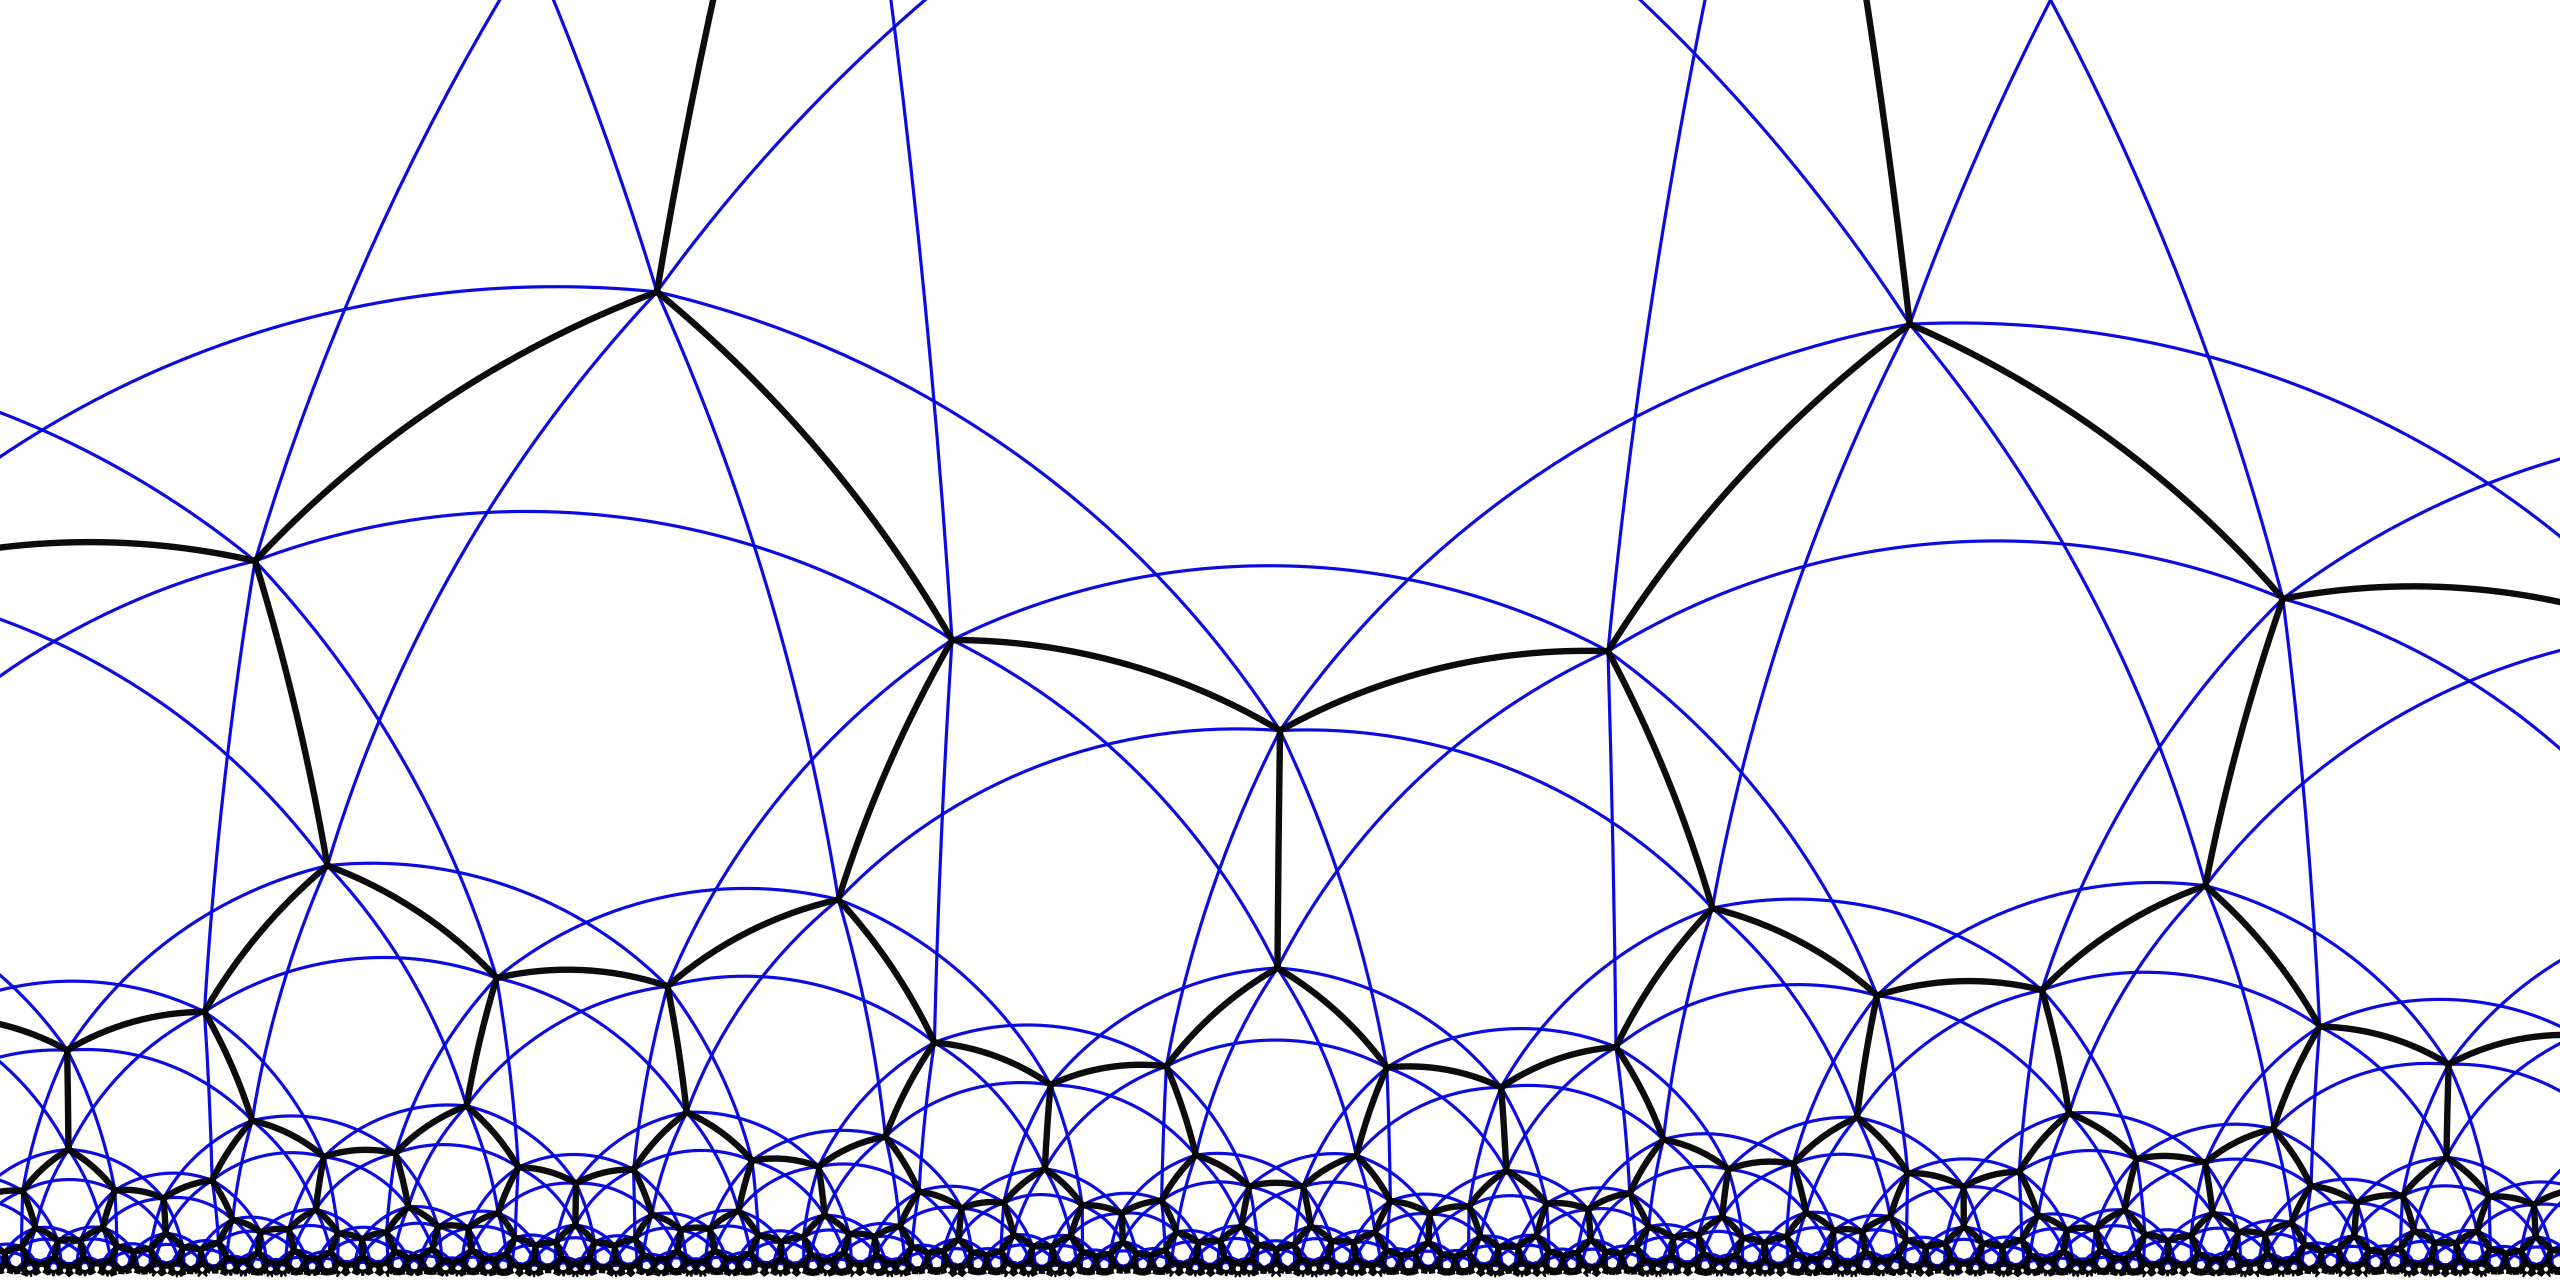
\includegraphics[width=0.9\textwidth]{~/Tesis/Figuras/A-Figuras/GeodesicasSemiPlano.png}
	\caption{Figura}
\end{figure}
